\clearpage
\cleardoublepage

\chapter{Mathematical Foundations}

\section{Introduction}

Neural networks are built upon a solid mathematical foundation that combines linear algebra, calculus, probability theory, and optimization. This chapter provides the essential mathematical prerequisites for understanding how neural networks learn and make predictions. We will cover these topics in the context of their applications in deep learning, providing both theoretical insights and practical intuitions.

The mathematics of neural networks can be viewed as the composition of linear transformations with nonlinear activation functions, optimized through gradient-based methods. Understanding this framework requires fluency in vector and matrix operations, differentiation of multivariate functions, and stochastic optimization.

\section{Linear Algebra}

Linear algebra provides the language for representing and manipulating data in neural networks. Neural networks fundamentally operate through linear transformations (matrix multiplications) combined with nonlinear activation functions.

\subsection{Vectors and Matrices}

A vector is an ordered collection of numbers that can represent a point in $n$-dimensional space. In neural networks, input data, hidden representations, and parameters are all represented as vectors or higher-dimensional tensors.

\begin{definition}[Vector]
A vector $\mathbf{x} \in \mathbb{R}^n$ is an ordered tuple of $n$ real numbers:
\begin{equation}
\mathbf{x} = \begin{bmatrix} x_1 \\ x_2 \\ \vdots \\ x_n \end{bmatrix} = (x_1, x_2, \ldots, x_n)^\top
\end{equation}
where $x_i$ denotes the $i$-th component of the vector.
\end{definition}

\begin{definition}[Matrix]
A matrix $\mathbf{A} \in \mathbb{R}^{m \times n}$ is a two-dimensional array of $m$ rows and $n$ columns:
\begin{equation}
\mathbf{A} = \begin{bmatrix}
a_{11} & a_{12} & \cdots & a_{1n} \\
a_{21} & a_{22} & \cdots & a_{2n} \\
\vdots & \vdots & \ddots & \vdots \\
a_{m1} & a_{m2} & \cdots & a_{mn}
\end{bmatrix}
\end{equation}
where $a_{ij}$ denotes the element in the $i$-th row and $j$-th column.
\end{definition}

\begin{example}[Neural Network Layer as Matrix Operation]
A single fully-connected layer in a neural network performs the operation:
\begin{equation}
\mathbf{y} = \mathbf{W}\mathbf{x} + \mathbf{b}
\end{equation}
where:
\begin{itemize}
    \item $\mathbf{x} \in \mathbb{R}^{d_{in}}$ is the input vector
    \item $\mathbf{W} \in \mathbb{R}^{d_{out} \times d_{in}}$ is the weight matrix
    \item $\mathbf{b} \in \mathbb{R}^{d_{out}}$ is the bias vector
    \item $\mathbf{y} \in \mathbb{R}^{d_{out}}$ is the output vector
\end{itemize}
If $d_{in} = 784$ (MNIST image) and $d_{out} = 128$, then $\mathbf{W}$ contains $784 \times 128 = 100,352$ parameters.
\end{example}

\subsection{Matrix Operations}

\begin{itemize}
    \item \textbf{Matrix Addition:} $\mathbf{C} = \mathbf{A} + \mathbf{B}$, where $c_{ij} = a_{ij} + b_{ij}$
    \item \textbf{Scalar Multiplication:} $c\mathbf{A}$, where every element is multiplied by $c$
    \item \textbf{Matrix Multiplication:} $\mathbf{C} = \mathbf{AB}$, where $c_{ij} = \sum_{k} a_{ik}b_{kj}$
    \item \textbf{Transpose:} $(\mathbf{A}^\top)_{ij} = a_{ji}$
    \item \textbf{Element-wise (Hadamard) Product:} $(\mathbf{A} \odot \mathbf{B})_{ij} = a_{ij} \cdot b_{ij}$
\end{itemize}

\begin{property}[Matrix Multiplication Properties]
For matrices $\mathbf{A}$, $\mathbf{B}$, and $\mathbf{C}$ of appropriate dimensions:
\begin{align}
\mathbf{A}(\mathbf{BC}) &= (\mathbf{AB})\mathbf{C} \quad \text{(associativity)} \\
\mathbf{A}(\mathbf{B} + \mathbf{C}) &= \mathbf{AB} + \mathbf{AC} \quad \text{(distributivity)} \\
(\mathbf{AB})^\top &= \mathbf{B}^\top \mathbf{A}^\top \quad \text{(transpose of product)}
\end{align}
Note: $\mathbf{AB} \neq \mathbf{BA}$ in general (non-commutativity).
\end{property}

\subsection{Norms}

Norms measure the ``size'' or ``length'' of vectors and matrices.

\begin{definition}[Vector Norms]
For a vector $\mathbf{x} \in \mathbb{R}^n$:
\begin{itemize}
    \item $L_1$ norm (Manhattan norm): $\|\mathbf{x}\|_1 = \sum_{i=1}^{n} |x_i|$
    \item $L_2$ norm (Euclidean norm): $\|\mathbf{x}\|_2 = \sqrt{\sum_{i=1}^{n} x_i^2}$
    \item $L_p$ norm: $\|\mathbf{x}\|_p = \left(\sum_{i=1}^{n} |x_i|^p\right)^{1/p}$
    \item $L_\infty$ norm (max norm): $\|\mathbf{x}\|_\infty = \max_i |x_i|$
\end{itemize}
\end{definition}

In neural networks, the $L_2$ norm is commonly used in regularization (weight decay), while the $L_1$ norm promotes sparsity.

\begin{example}[Weight Decay Regularization]
Weight decay adds a penalty term to the loss function:
\begin{equation}
\mathcal{L}_{reg}(\mathbf{W}) = \mathcal{L}(\mathbf{W}) + \lambda \|\mathbf{W}\|_F^2
\end{equation}
where $\|\mathbf{W}\|_F = \sqrt{\sum_{i,j} w_{ij}^2}$ is the Frobenius norm (the $L_2$ norm of the flattened matrix).
\end{example}

\subsection{Eigenvalues and Singular Values}

Eigenvalues and singular values are fundamental for understanding linear transformations, dimensionality reduction, and network analysis.

\begin{definition}[Eigenvalue and Eigenvector]
For a square matrix $\mathbf{A} \in \mathbb{R}^{n \times n}$, if there exists a scalar $\lambda$ and nonzero vector $\mathbf{v}$ such that:
\begin{equation}
\mathbf{A}\mathbf{v} = \lambda \mathbf{v}
\end{equation}
then $\lambda$ is called an eigenvalue and $\mathbf{v}$ is the corresponding eigenvector.
\end{definition}

\begin{definition}[Singular Value Decomposition]
For any matrix $\mathbf{A} \in \mathbb{R}^{m \times n}$, the Singular Value Decomposition (SVD) is:
\begin{equation}
\mathbf{A} = \mathbf{U}\Sigma\mathbf{V}^\top
\end{equation}
where:
\begin{itemize}
    \item $\mathbf{U} \in \mathbb{R}^{m \times m}$ and $\mathbf{V} \in \mathbb{R}^{n \times n}$ are orthogonal matrices
    \item $\Sigma \in \mathbb{R}^{m \times n}$ is a diagonal matrix containing singular values $\sigma_1 \geq \sigma_2 \geq \cdots \geq 0$
\end{itemize}
The singular values are related to eigenvalues by $\sigma_i = \sqrt{\lambda_i(\mathbf{A}^\top\mathbf{A})}$.
\end{definition}

SVD is crucial for Principal Component Analysis (PCA), which is used in understanding the dimensionality of neural network representations.

\subsubsection{Why SVD Matters: Geometric Interpretation}

To understand why SVD is so fundamental, consider the geometric action of a matrix $\mathbf{A}$. The equation $\mathbf{y} = \mathbf{A}\mathbf{x}$ can be decomposed into three sequential transformations via SVD:
\begin{enumerate}
    \item $\mathbf{V}^\top$: Rotate (or reflect) the input vector into the ``right singular basis.''
    \item $\Sigma$: Scale along each axis by the corresponding singular value $\sigma_i$.
    \item $\mathbf{U}$: Rotate into the ``left singular basis'' for the output space.
\end{enumerate}
This geometric view reveals that the singular values $\sigma_1 \geq \sigma_2 \geq \cdots \geq 0$ describe exactly how much $\mathbf{A}$ stretches space along each principal direction. In neural networks, the weight matrix $\mathbf{W}$ of a layer performs exactly this kind of transformation on the input activations.

\begin{figure}[htbp]
    \centering
    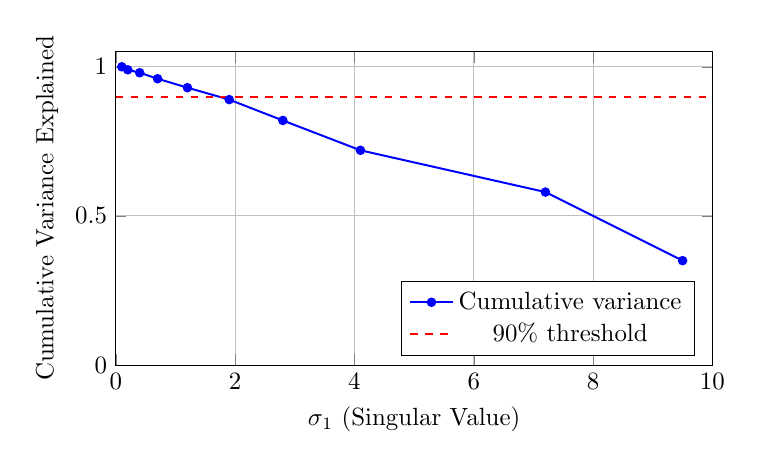
\begin{tikzpicture}[scale=0.9]
        \begin{axis}[
            xlabel={$\sigma_1$ (Singular Value)},
            ylabel={Cumulative Variance Explained},
            xmin=0, xmax=10,
            ymin=0, ymax=1.05,
            width=10cm,
            height=6cm,
            legend pos=south east,
            grid=major
        ]
            \addplot[thick, blue, mark=*, mark size=1.5pt] coordinates {
                (9.5, 0.35) (7.2, 0.58) (4.1, 0.72) (2.8, 0.82)
                (1.9, 0.89) (1.2, 0.93) (0.7, 0.96) (0.4, 0.98)
                (0.2, 0.99) (0.1, 1.0)
            };
            \addlegendentry{Cumulative variance}
            \addplot[dashed, red, thick] coordinates {(0, 0.9) (10, 0.9)};
            \addlegendentry{90\% threshold}
        \end{axis}
    \end{tikzpicture}
    \caption[Singular value spectrum]{Typical singular value spectrum of a neural network weight matrix. Most variance is captured by the top few singular values, motivating low-rank approximations.}
    \label{fig:svd_spectrum}
\end{figure}

\subsubsection{Low-Rank Approximation: The Eckart--Young Theorem}

One of the most powerful applications of SVD in deep learning is low-rank approximation. Given a rank-$r$ approximation $\hat{\mathbf{A}}_r = \sum_{i=1}^{r} \sigma_i \mathbf{u}_i \mathbf{v}_i^\top$, the Eckart--Young theorem guarantees:

\begin{theorem}[Eckart--Young--Mirsky, 1936/1949]
For any matrix $\mathbf{A} \in \mathbb{R}^{m \times n}$ with SVD $\mathbf{A} = \mathbf{U}\Sigma\mathbf{V}^\top$, the best rank-$r$ approximation in both the spectral norm and Frobenius norm is given by keeping the top $r$ singular values:
\begin{equation}
\hat{\mathbf{A}}_r = \arg\min_{\text{rank}(\mathbf{B}) \leq r} \|\mathbf{A} - \mathbf{B}\|_F = \sum_{i=1}^{r} \sigma_i \mathbf{u}_i \mathbf{v}_i^\top
\end{equation}
with approximation error $\|\mathbf{A} - \hat{\mathbf{A}}_r\|_F = \sqrt{\sum_{i=r+1}^{\min(m,n)} \sigma_i^2}$.
\end{theorem}

This theorem underpins modern techniques such as \textbf{LoRA} (Low-Rank Adaptation) for efficient fine-tuning of large language models \cite{hu2021lora}, where the weight update $\Delta\mathbf{W}$ is parameterized as a product $\mathbf{B}\mathbf{A}$ with rank $r \ll \min(m, n)$, reducing trainable parameters from $mn$ to $(m + n)r$.

\subsubsection{Eigendecomposition and Spectral Theorem}

For symmetric matrices (which arise frequently as Hessian matrices $\mathbf{H}$ in optimization), the eigendecomposition takes a special, simplified form:

\begin{theorem}[Spectral Theorem]
For any real symmetric matrix $\mathbf{A} \in \mathbb{R}^{n \times n}$ ($\mathbf{A} = \mathbf{A}^\top$), there exists an orthogonal matrix $\mathbf{Q}$ and a diagonal matrix $\Lambda$ such that:
\begin{equation}
\mathbf{A} = \mathbf{Q}\Lambda\mathbf{Q}^\top = \sum_{i=1}^{n} \lambda_i \mathbf{q}_i \mathbf{q}_i^\top
\end{equation}
where $\lambda_1 \geq \lambda_2 \geq \cdots \geq \lambda_n$ are real eigenvalues and $\mathbf{q}_i$ are orthonormal eigenvectors.
\end{theorem}

The Hessian $\mathbf{H} = \nabla^2 \mathcal{L}(\boldsymbol{\theta})$ of a loss function is always symmetric (by Clairaut's theorem on equality of mixed partials). Its eigenvalues determine the local geometry of the loss surface:
\begin{itemize}
    \item All $\lambda_i > 0$: local minimum (positive definite)
    \item All $\lambda_i < 0$: local maximum (negative definite)
    \item Mixed signs: saddle point (indefinite)
\end{itemize}

\subsubsection{Condition Number and Numerical Stability}

The condition number of a matrix measures how sensitive the solution of $\mathbf{A}\mathbf{x} = \mathbf{b}$ is to perturbations in $\mathbf{b}$:

\begin{definition}[Condition Number]
The condition number of a matrix $\mathbf{A}$ (with respect to the $L_2$ norm) is:
\begin{equation}
\kappa(\mathbf{A}) = \|\mathbf{A}\|_2 \cdot \|\mathbf{A}^{-1}\|_2 = \frac{\sigma_{\max}(\mathbf{A})}{\sigma_{\min}(\mathbf{A})}
\end{equation}
For a symmetric positive definite matrix, $\kappa(\mathbf{A}) = \lambda_{\max} / \lambda_{\min}$.
\end{definition}

In gradient descent, the condition number of the Hessian $\kappa(\mathbf{H})$ directly bounds the convergence rate. For a quadratic objective $\mathcal{L}(\boldsymbol{\theta}) = \frac{1}{2}\boldsymbol{\theta}^\top \mathbf{H}\boldsymbol{\theta} - \mathbf{b}^\top\boldsymbol{\theta}$, gradient descent with learning rate $\alpha$ converges if and only if:
\begin{equation}
0 < \alpha < \frac{2}{\lambda_{\max}}
\end{equation}
and the optimal learning rate is $\alpha^* = \frac{2}{\lambda_{\max} + \lambda_{\min}}$, giving a convergence rate:
\begin{equation}
\left(\frac{\kappa(\mathbf{H}) - 1}{\kappa(\mathbf{H}) + 1}\right)^2
\end{equation}
per iteration. When $\kappa(\mathbf{H}) \gg 1$ (ill-conditioned), convergence becomes extremely slow---this is a fundamental motivation for adaptive optimizers like Adam (Chapter~7), which effectively rescale the gradient along each dimension.

\begin{figure}[htbp]
    \centering
    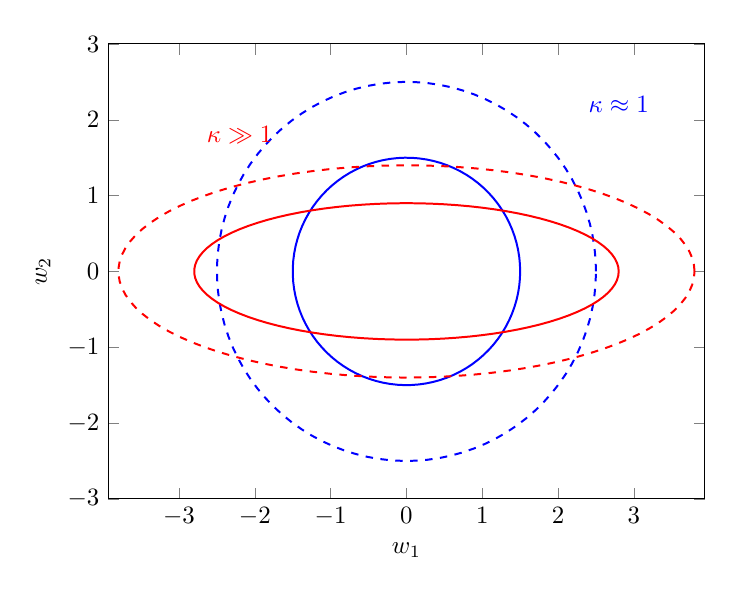
\begin{tikzpicture}[scale=0.9]
        \begin{axis}[
            xlabel={$w_1$},
            ylabel={$w_2$},
            width=10cm,
            height=8cm,
            axis equal,
            xmin=-3, xmax=3,
            ymin=-3, ymax=3,
        ]
            % Well-conditioned (kappa ~ 1)
            \addplot[blue, thick, domain=0:360, samples=100]
                ({1.5*cos(x)}, {1.5*sin(x)});
            \addplot[blue, thick, dashed, domain=0:360, samples=100]
                ({2.5*cos(x)}, {2.5*sin(x)});
            \node[blue] at (axis cs:2.8, 2.2) {$\kappa \approx 1$};
            
            % Ill-conditioned (kappa ~ 10)
            \addplot[red, thick, domain=0:360, samples=100]
                ({2.8*cos(x)}, {0.9*sin(x)});
            \addplot[red, thick, dashed, domain=0:360, samples=100]
                ({3.8*cos(x)}, {1.4*sin(x)});
            \node[red] at (axis cs:-2.2, 1.8) {$\kappa \gg 1$};
        \end{axis}
    \end{tikzpicture}
    \caption[Condition number and loss contours]{Loss contours for well-conditioned (circular, $\kappa \approx 1$) and ill-conditioned (elliptical, $\kappa \gg 1$) problems. Gradient descent zigzags on ill-conditioned landscapes.}
    \label{fig:condition_number}
\end{figure}

\subsubsection{Positive Definite Matrices and Cholesky Decomposition}

\begin{definition}[Positive Definite]
A symmetric matrix $\mathbf{A}$ is positive definite if $\mathbf{x}^\top \mathbf{A}\mathbf{x} > 0$ for all nonzero $\mathbf{x}$.
\end{definition}

For covariance matrices (which are always positive semidefinite), the Cholesky decomposition provides an efficient factorization:

\begin{theorem}[Cholesky Decomposition]
For any symmetric positive definite $\mathbf{A} \in \mathbb{R}^{n \times n}$:
\begin{equation}
\mathbf{A} = \mathbf{L}\mathbf{L}^\top
\end{equation}
where $\mathbf{L}$ is a lower triangular matrix with positive diagonal entries. Computation requires $\frac{n^3}{6}$ FLOPs, half that of LU decomposition.
\end{theorem}

The Cholesky decomposition is essential for:
\begin{itemize}
    \item \textbf{Sampling from multivariate Gaussians:} If $\mathbf{x} \sim \mathcal{N}(\boldsymbol{\mu}, \boldsymbol{\Sigma})$, then $\mathbf{x} = \boldsymbol{\mu} + \mathbf{L}\mathbf{z}$ where $\mathbf{z} \sim \mathcal{N}(\mathbf{0}, \mathbf{I})$ and $\boldsymbol{\Sigma} = \mathbf{L}\mathbf{L}^\top$.
    \item \textbf{Kalman filters} and \textbf{variational inference} in probabilistic deep learning.
    \item \textbf{Solving linear systems} $\mathbf{A}\mathbf{x} = \mathbf{b}$ in optimization subroutines.
\end{itemize}

\subsubsection{Determinant, Trace, and Jacobian Determinant}

Two scalar summaries of a matrix that appear frequently in deep learning:

\begin{property}[Key Matrix Properties]
For an $n \times n$ matrix $\mathbf{A}$ with eigenvalues $\lambda_1, \ldots, \lambda_n$:
\begin{align}
\det(\mathbf{A}) &= \prod_{i=1}^{n} \lambda_i = \text{signed volume scaling factor} \\
\text{tr}(\mathbf{A}) &= \sum_{i=1}^{n} \lambda_i = \sum_{i=1}^{n} a_{ii} \\
\det(\mathbf{A}) &= \exp(\text{tr}(\log \mathbf{A})) \quad \text{(matrix log identity)}
\end{align}
\end{property}

The \textbf{Jacobian determinant} is crucial in normalizing flows and variational autoencoders (VAEs). If $\mathbf{y} = g(\mathbf{x})$ is an invertible transformation, then by the change of variables formula:
\begin{equation}
p_{\mathbf{Y}}(\mathbf{y}) = p_{\mathbf{X}}(g^{-1}(\mathbf{y})) \cdot \left|\det \frac{\partial g^{-1}(\mathbf{y})}{\partial \mathbf{y}}\right| = p_{\mathbf{X}}(\mathbf{x}) \cdot \left|\det \frac{\partial g(\mathbf{x})}{\partial \mathbf{x}}\right|^{-1}
\end{equation}
Normalizing flows design $g$ so that this determinant is cheap to compute, enabling exact likelihood evaluation. Variational autoencoders and normalizing flows for generative modeling are discussed later in this book.

\subsection{Tensors}

Neural networks, especially convolutional neural networks, operate on higher-dimensional arrays called tensors.

\begin{definition}[Tensor]
A tensor is a generalization of vectors and matrices to higher dimensions:
\begin{itemize}
    \item 0D tensor: scalar
    \item 1D tensor: vector
    \item 2D tensor: matrix
    \item 3D tensor: e.g., RGB images of shape $(H, W, C)$
    \item 4D tensor: batches of images of shape $(N, H, W, C)$
    \item 5D tensor: volumes of shape $(D, H, W, C)$
\end{itemize}
\end{definition}

\begin{example}[Tensor Shapes in CNNs]
For a batch of $N$ color images of size $H \times W$ with 3 channels (RGB):
\begin{itemize}
    \item Input tensor: $\mathbf{X} \in \mathbb{R}^{N \times H \times W \times 3}$
    \item After convolution with $C$ filters: $\mathbf{Y} \in \mathbb{R}^{N \times H' \times W' \times C}$
\end{itemize}
PyTorch convention: $(N, C, H, W)$
TensorFlow convention: $(N, H, W, C)$
\end{example}

\section{Calculus}

Calculus, particularly differential calculus, is essential for understanding how neural networks learn through gradient-based optimization.

\subsection{Derivatives and Gradients}

\begin{definition}[Derivative]
The derivative of a function $f: \mathbb{R} \to \mathbb{R}$ at point $x$ is defined as:
\begin{equation}
f'(x) = \frac{df}{dx} = \lim_{h \to 0} \frac{f(x + h) - f(x)}{h}
\end{equation}
\end{definition}

\begin{definition}[Gradient]
For a scalar function $f: \mathbb{R}^n \to \mathbb{R}$, the gradient is a vector of partial derivatives:
\begin{equation}
\nabla f(\mathbf{x}) = \begin{bmatrix}
\frac{\partial f}{\partial x_1} \\
\frac{\partial f}{\partial x_2} \\
\vdots \\
\frac{\partial f}{\partial x_n}
\end{bmatrix}
\end{equation}
The gradient points in the direction of steepest ascent.
\end{definition}

\begin{property}[Rules of Differentiation]
\begin{itemize}
    \item Sum rule: $\frac{d}{dx}(f + g) = f' + g'$
    \item Product rule: $\frac{d}{dx}(fg) = f'g + fg'$
    \item Chain rule: $\frac{d}{dx}f(g(x)) = f'(g(x)) \cdot g'(x)$
    \item Quotient rule: $\frac{d}{dx}\left(\frac{f}{g}\right) = \frac{f'g - fg'}{g^2}$
\end{itemize}
\end{property}

\begin{example}[Chain Rule in Neural Networks]
For a two-layer network $f(\mathbf{x}) = \mathbf{W}_2(\mathbf{W}_1\mathbf{x} + \mathbf{b}_1) + \mathbf{b}_2$, the gradient computation uses the chain rule extensively. If we want $\frac{\partial \mathcal{L}}{\partial \mathbf{W}_1}$ for loss $\mathcal{L}$, we have:
\begin{equation}
\frac{\partial \mathcal{L}}{\partial \mathbf{W}_1} = \frac{\partial \mathcal{L}}{\partial \mathbf{z}_2} \cdot \frac{\partial \mathbf{z}_2}{\partial \mathbf{z}_1} \cdot \frac{\partial \mathbf{z}_1}{\partial \mathbf{W}_1}
\end{equation}
where $\mathbf{z}_1 = \mathbf{W}_1\mathbf{x} + \mathbf{b}_1$ and $\mathbf{z}_2 = \mathbf{W}_2\mathbf{z}_1 + \mathbf{b}_2$.
\end{example}

\subsection{Higher-Order Derivatives}

\begin{definition}[Hessian Matrix]
For a function $f: \mathbb{R}^n \to \mathbb{R}$, the Hessian matrix contains all second-order partial derivatives:
\begin{equation}
\mathbf{H} = \nabla^2 f(\mathbf{x}) = \begin{bmatrix}
\frac{\partial^2 f}{\partial x_1^2} & \frac{\partial^2 f}{\partial x_1 \partial x_2} & \cdots \\
\frac{\partial^2 f}{\partial x_2 \partial x_1} & \frac{\partial^2 f}{\partial x_2^2} & \cdots \\
\vdots & \vdots & \ddots
\end{bmatrix}
\end{equation}
The Hessian is symmetric if all second derivatives are continuous.
\end{definition}

The Hessian is used in Newton's method and for understanding curvature of the loss landscape.

\subsubsection{Taylor Expansion: The Theoretical Bridge}

The Taylor expansion is the single most important mathematical tool connecting first-order and second-order optimization methods. For a twice-differentiable function $f: \mathbb{R}^n \to \mathbb{R}$ around point $\mathbf{a}$:

\begin{definition}[Multivariate Taylor Expansion]
\begin{align}
f(\mathbf{a} + \boldsymbol{\delta}) &= f(\mathbf{a}) + \nabla f(\mathbf{a})^\top \boldsymbol{\delta} + \frac{1}{2}\boldsymbol{\delta}^\top \mathbf{H}(\mathbf{a})\boldsymbol{\delta} + \mathcal{O}(\|\boldsymbol{\delta}\|^3)
\end{align}
where $\nabla f(\mathbf{a})$ is the gradient and $\mathbf{H}(\mathbf{a}) = \nabla^2 f(\mathbf{a})$ is the Hessian evaluated at $\mathbf{a}$.
\end{definition}

\textbf{Why this matters for neural networks:} Nearly all optimization theory can be understood through the lens of local Taylor approximation.

\begin{example}[Gradient Descent as First-Order Taylor Approximation]
Setting $\boldsymbol{\delta} = -\alpha \nabla f(\mathbf{a})$ in the first-order expansion:
\begin{equation}
f(\mathbf{a} - \alpha \nabla f(\mathbf{a})) \approx f(\mathbf{a}) - \alpha \|\nabla f(\mathbf{a})\|^2
\end{equation}
This guarantees descent as long as $\alpha > 0$ and the linear approximation is valid---i.e., $\alpha$ is not too large.
\end{example}

\begin{example}[Newton's Method as Second-Order Approximation]
Minimizing the second-order Taylor approximation:
\begin{equation}
f(\mathbf{a} + \boldsymbol{\delta}) \approx f(\mathbf{a}) + \nabla f(\mathbf{a})^\top \boldsymbol{\delta} + \frac{1}{2}\boldsymbol{\delta}^\top \mathbf{H}\boldsymbol{\delta}
\end{equation}
Setting the gradient with respect to $\boldsymbol{\delta}$ to zero:
\begin{equation}
\nabla f(\mathbf{a}) + \mathbf{H}\boldsymbol{\delta}^* = 0 \implies \boldsymbol{\delta}^* = -\mathbf{H}^{-1}\nabla f(\mathbf{a})
\end{equation}
This is Newton's update. It converges quadratically near a minimum but requires $\mathcal{O}(n^3)$ per step for the matrix inverse---prohibitive for deep networks with millions of parameters. Modern quasi-Newton methods (L-BFGS) and approximate second-order methods (K-FAC, Shampoo) attempt to capture curvature information at manageable cost.
\end{example}

\subsubsection{Convexity and the Loss Landscape}

Convexity determines whether gradient descent can find the global minimum:

\begin{definition}[Convex Function]
A function $f$ is \textbf{convex} if for all $\mathbf{x}, \mathbf{y}$ and $\lambda \in [0,1]$:
\begin{equation}
f(\lambda \mathbf{x} + (1-\lambda)\mathbf{y}) \leq \lambda f(\mathbf{x}) + (1-\lambda)f(\mathbf{y})
\end{equation}
\end{definition}

\begin{definition}[Strongly Convex Function]
A twice-differentiable $f$ is $\mu$-strongly convex if:
\begin{equation}
\nabla^2 f(\mathbf{x}) \succeq \mu \mathbf{I} \quad \text{(all eigenvalues of Hessian $\geq \mu > 0$)}
\end{equation}
\end{definition}

\textbf{The bad news:} Neural network loss landscapes are \emph{non-convex}---the Hessian has both positive and negative eigenvalues everywhere. However, a remarkable empirical finding is that \textbf{most local minima in overparameterized networks have similar loss values} \cite{choromanska2015loss}, and the dominant challenge is saddle points rather than poor local minima.

\begin{table}[ht]
    \centering
    \caption{Convexity Properties and Their Implications for Optimization}
    \begin{tabular}{L{3.5cm} L{4cm} L{5cm}}
        \toprule
        \textbf{Property} & \textbf{Condition} & \textbf{Implication} \\
        \midrule
        Convex & $\nabla^2 f \succeq 0$ & All local minima are global \\
        Strictly convex & $\nabla^2 f \succ 0$ & Unique global minimum \\
        $\mu$-strongly convex & $\nabla^2 f \succeq \mu\mathbf{I}$ & Linear convergence rate \\
        $L$-smooth & $\|\nabla^2 f\| \leq L$ & Descent guaranteed for $\alpha < 2/L$ \\
        $PL$ condition & -- & Linear convergence even if non-convex \\
        \bottomrule
    \end{tabular}
\end{table}

The Polyak--\L{}ojasiewicz (PL) condition is a relaxation of strong convexity that applies to some non-convex problems:
\begin{equation}
\frac{1}{2}\|\nabla f(\mathbf{x})\|^2 \geq \mu(f(\mathbf{x}) - f^*)
\end{equation}
where $f^*$ is the optimal value. Many neural network training objectives are conjectured to approximately satisfy this condition, explaining why gradient descent often finds good solutions despite non-convexity.

\subsubsection{Lipschitz Continuity and Gradient Clipping}

\begin{definition}[$L$-Lipschitz Continuous]
A function $f$ is $L$-Lipschitz continuous if:
\begin{equation}
|f(\mathbf{x}) - f(\mathbf{y})| \leq L\|\mathbf{x} - \mathbf{y}\| \quad \forall \mathbf{x}, \mathbf{y}
\end{equation}
Equivalently, $\|\nabla f(\mathbf{x})\| \leq L$ for differentiable $f$.
\end{definition}

In neural networks, the Lipschitz constant of each layer bounds how much a small change in the input can affect the output. For a linear layer $\mathbf{y} = \mathbf{W}\mathbf{x}$, the Lipschitz constant equals $\|\mathbf{W}\|_2 = \sigma_{\max}(\mathbf{W})$.

\textbf{Gradient clipping} in RNNs and transformers limits the gradient norm:
\begin{equation}
\mathbf{g} \leftarrow \begin{cases}
\mathbf{g} & \text{if } \|\mathbf{g}\| \leq \tau \\
\frac{\tau}{\|\mathbf{g}\|} \mathbf{g} & \text{otherwise}
\end{cases}
\end{equation}
This prevents gradient explosion, which is particularly problematic for recurrent architectures and large language models.

\begin{example}[Gradient Descent vs. Newton's Method]
\begin{itemize}
    \item Gradient descent: $\mathbf{w}_{t+1} = \mathbf{w}_t - \alpha \nabla \mathcal{L}(\mathbf{w}_t)$
    \item Newton's method: $\mathbf{w}_{t+1} = \mathbf{w}_t - \alpha \mathbf{H}^{-1} \nabla \mathcal{L}(\mathbf{w}_t)$
\end{itemize}
Newton's method uses second-order information (curvature) for potentially faster convergence, but computing the Hessian is expensive for large networks.
\end{example}

\subsection{Jacobian Matrix}

\begin{definition}[Jacobian]
For a vector-valued function $\mathbf{f}: \mathbb{R}^n \to \mathbb{R}^m$, the Jacobian is an $m \times n$ matrix of partial derivatives:
\begin{equation}
\mathbf{J} = \frac{\partial \mathbf{f}}{\partial \mathbf{x}} = \begin{bmatrix}
\frac{\partial f_1}{\partial x_1} & \frac{\partial f_1}{\partial x_2} & \cdots \\
\frac{\partial f_2}{\partial x_1} & \frac{\partial f_2}{\partial x_2} & \cdots \\
\vdots & \vdots & \ddots
\end{bmatrix}
\end{equation}
Each row $i$ is the gradient of $f_i$.
\end{definition}

The Jacobian generalizes the gradient to vector-valued functions, which is essential for backpropagation through complex computational graphs.

\begin{example}[Jacobian in Backpropagation]
In backpropagation, we compute gradients of scalar outputs (like loss) with respect to vector inputs. If $\mathbf{y} = f(\mathbf{x})$ and $L$ is a scalar loss, then:
\begin{equation}
\frac{\partial L}{\partial \mathbf{x}} = \left(\frac{\partial \mathbf{y}}{\partial \mathbf{x}}\right)^\top \frac{\partial L}{\partial \mathbf{y}} = \mathbf{J}^\top \nabla_{\mathbf{y}} L
\end{equation}
The backward pass efficiently computes this product without explicitly forming the full Jacobian.
\end{example}

\section{Probability Theory}

Probability theory provides the framework for understanding uncertainty, making predictions, and designing loss functions.

\subsection{Basic Probability}

\begin{definition}[Probability]
For a random experiment with sample space $\Omega$, a probability function $P$ assigns to each event $A \subseteq \Omega$ a number $P(A)$ such that:
\begin{itemize}
    \item $0 \leq P(A) \leq 1$ for all events $A$
    \item $P(\Omega) = 1$
    \item If $A_1, A_2, \ldots$ are mutually exclusive, then $P(\bigcup_i A_i) = \sum_i P(A_i)$
\end{itemize}
\end{definition}

\begin{definition}[Random Variable]
A random variable $X$ is a function that maps outcomes of a random experiment to numerical values:
\begin{itemize}
    \item Discrete: $P(X = x)$ for countable values
    \item Continuous: described by probability density function $p(x)$
\end{itemize}
\end{definition}

\begin{itemize}
    \item \textbf{Expected Value:} $E[X] = \sum_x x \cdot P(X=x)$ or $\int x \cdot p(x) dx$
    \item \textbf{Variance:} $\text{Var}(X) = E[(X - E[X])^2] = E[X^2] - (E[X])^2$
    \item \textbf{Standard Deviation:} $\sigma_X = \sqrt{\text{Var}(X)}$
\end{itemize}

\subsection{Common Distributions}

\begin{table}[ht]
    \centering
    \caption{Common Probability Distributions in Deep Learning}
    \begin{tabular}{L{3cm} L{4cm} L{5cm}}
        \toprule
        \textbf{Distribution} & \textbf{Formula} & \textbf{Applications} \\
        \midrule
        Bernoulli & $P(X=1) = p, P(X=0) = 1-p$ & Binary classification \\
        Categorical & $P(X=k) = p_k$ & Multi-class classification \\
        Gaussian (Normal) & $p(x) = \frac{1}{\sqrt{2\pi\sigma^2}}e^{-\frac{(x-\mu)^2}{2\sigma^2}}$ & Regression, weight initialization \\
        Multinomial & Generalization of Bernoulli & Language modeling \\
        \bottomrule
    \end{tabular}
\end{table}

\begin{example}[Softmax Distribution]
The softmax function converts a vector of logits $\mathbf{z} \in \mathbb{R}^K$ into a probability distribution:
\begin{equation}
\text{softmax}(z_i) = \frac{e^{z_i}}{\sum_{j=1}^{K} e^{z_j}}
\end{equation}
Properties:
\begin{itemize}
    \item $\sum_{i=1}^{K} \text{softmax}(z_i) = 1$
    \item $\text{softmax}(z_i) \in (0, 1)$ for all $i$
    \item $\arg\max_i \text{softmax}(z_i) = \arg\max_i z_i$
\end{itemize}
Used for multi-class classification output.
\end{example}

\subsection{Bayesian Probability}

\begin{definition}[Bayes' Rule]
\begin{equation}
P(A|B) = \frac{P(B|A) \cdot P(A)}{P(B)}
\end{equation}
In the context of machine learning:
\begin{equation}
P(\text{hypothesis}|\text{data}) = \frac{P(\text{data}|\text{hypothesis}) \cdot P(\text{hypothesis})}{P(\text{data})}
\end{equation}
\begin{itemize}
    \item $P(\text{hypothesis})$: Prior probability
    \item $P(\text{data}|\text{hypothesis})$: Likelihood
    \item $P(\text{hypothesis}|\text{data})$: Posterior probability
\end{itemize}
\end{definition}

Bayesian methods are used in Bayesian neural networks for uncertainty estimation and in Bayesian optimization for hyperparameter tuning.

\subsection{Maximum Likelihood Estimation}

Maximum Likelihood Estimation (MLE) is the statistical principle underlying most loss functions in deep learning.

\begin{definition}[Maximum Likelihood Estimation]
Given a dataset $\mathcal{D} = \{(\mathbf{x}_i, y_i)\}_{i=1}^{N}$ drawn i.i.d.\ from an unknown distribution, MLE finds the parameter $\theta$ that maximizes the probability of observing the data:
\begin{equation}
\theta_{\text{MLE}} = \arg\max_{\theta} \prod_{i=1}^{N} p(y_i \mid \mathbf{x}_i; \theta)
\end{equation}
Equivalently (taking the negative log for numerical stability):
\begin{equation}
\theta_{\text{MLE}} = \arg\min_{\theta} \underbrace{-\sum_{i=1}^{N} \log p(y_i \mid \mathbf{x}_i; \theta)}_{\text{Negative Log-Likelihood (NLL)}}
\end{equation}
\end{definition}

The negative log-likelihood (NLL) \emph{is} the loss function. Different model assumptions lead to different loss functions:

\begin{example}[MSE as MLE under Gaussian Noise]
Assume $y = f(\mathbf{x}; \theta) + \epsilon$ where $\epsilon \sim \mathcal{N}(0, \sigma^2)$. Then:
\begin{align}
p(y \mid \mathbf{x}; \theta) &= \frac{1}{\sqrt{2\pi\sigma^2}} \exp\left(-\frac{(y - f(\mathbf{x};\theta))^2}{2\sigma^2}\right) \\
-\log p(y \mid \mathbf{x}; \theta) &= \frac{(y - \hat{y})^2}{2\sigma^2} + \frac{1}{2}\log(2\pi\sigma^2)
\end{align}
Since the constant $\frac{1}{2}\log(2\pi\sigma^2)$ does not depend on $\theta$, minimizing NLL is equivalent to minimizing MSE. This explains why MSE is the ``natural'' loss for regression---it corresponds to the assumption of additive Gaussian noise.

The gradient of the MSE loss:
\begin{equation}
\frac{\partial \mathcal{L}_{\text{MSE}}}{\partial \hat{y}} = \frac{2}{N}(\hat{y} - y)
\end{equation}
is proportional to the residual, meaning large errors receive proportionally large gradients---this is both a strength (fast convergence near the optimum) and a weakness (sensitivity to outliers).
\end{example}

\begin{example}[Cross-Entropy as MLE for Categorical Distributions]
For $K$-class classification, model the output as a categorical distribution:
\begin{equation}
p(y = k \mid \mathbf{x}; \theta) = \hat{y}_k = \text{softmax}(\mathbf{z})_k
\end{equation}
The negative log-likelihood becomes:
\begin{equation}
\mathcal{L}_{\text{NLL}} = -\sum_{k=1}^{K} y_k \log \hat{y}_k = -\log \hat{y}_{c}
\end{equation}
where $c$ is the true class. This is exactly the cross-entropy loss. The gradient simplifies beautifully:
\begin{equation}
\frac{\partial \mathcal{L}}{\partial z_k} = \hat{y}_k - y_k
\end{equation}
The gradient is simply the difference between prediction and target---the ``error signal.'' This clean form is one reason softmax + cross-entropy is the standard for classification.
\end{example}

\subsection{Bayesian Inference and MAP Estimation}

While MLE finds the single best parameter, Bayesian inference treats the parameter $\theta$ itself as a random variable with a prior distribution $p(\theta)$.

\begin{definition}[Maximum A Posteriori (MAP) Estimation]
\begin{equation}
\theta_{\text{MAP}} = \arg\max_{\theta} \; p(\theta \mid \mathcal{D}) = \arg\max_{\theta} \; \underbrace{\log p(\mathcal{D} \mid \theta)}_{\text{log-likelihood}} + \underbrace{\log p(\theta)}_{\text{log-prior}}
\end{equation}
\end{definition}

\begin{example}[Weight Decay as MAP with Gaussian Prior]
If we place a Gaussian prior $\theta_j \sim \mathcal{N}(0, \lambda^{-1})$ on each weight, then:
\begin{equation}
\log p(\theta) = \sum_j \log \frac{1}{\sqrt{2\pi/\lambda}} \exp\left(-\frac{\lambda \theta_j^2}{2}\right) = -\frac{\lambda}{2}\|\theta\|_2^2 + \text{const}
\end{equation}
Thus, MAP estimation with a Gaussian prior is equivalent to MLE with $L_2$ regularization (weight decay):
\begin{equation}
\theta_{\text{MAP}} = \arg\min_{\theta} \; \mathcal{L}(\theta) + \frac{\lambda}{2}\|\theta\|_2^2
\end{equation}
Similarly, a Laplace prior $p(\theta_j) \propto \exp(-\lambda|\theta_j|)$ gives $L_1$ regularization, promoting sparsity.
\end{example}

\subsection{Conjugate Priors and Exponential Families}

Many common distributions in deep learning belong to the \textbf{exponential family}:
\begin{equation}
p(\mathbf{x} \mid \boldsymbol{\eta}) = h(\mathbf{x}) \exp\left(\boldsymbol{\eta}^\top T(\mathbf{x}) - A(\boldsymbol{\eta})\right)
\end{equation}
where $\boldsymbol{\eta}$ are natural parameters, $T(\mathbf{x})$ are sufficient statistics, and $A(\boldsymbol{\eta})$ is the log-partition function.

\begin{property}[Conjugate Priors]
A prior $p(\boldsymbol{\eta})$ is conjugate to a likelihood $p(\mathbf{x} \mid \boldsymbol{\eta})$ if the posterior $p(\boldsymbol{\eta} \mid \mathbf{x})$ belongs to the same distribution family as the prior. Key examples:
\end{property}

\begin{table}[ht]
    \centering
    \caption{Common Conjugate Prior Relationships}
    \begin{tabular}{L{2.5cm} L{2.5cm} L{2.5cm} L{3cm}}
        \toprule
        \textbf{Likelihood} & \textbf{Prior} & \textbf{Posterior} & \textbf{Application} \\
        \midrule
        Bernoulli & Beta & Beta & Click-through rate \\
        Multinomial & Dirichlet & Dirichlet & Topic models (LDA) \\
        Gaussian (known $\sigma^2$) & Gaussian & Gaussian & Bayesian regression \\
        Gaussian (known $\mu$) & Inverse-Gamma & Inverse-Gamma & Variance estimation \\
        Poisson & Gamma & Gamma & Count data \\
        \bottomrule
    \end{tabular}
\end{table}

\section{Optimization}

Neural network training is fundamentally an optimization problem: finding parameters that minimize a loss function.

\subsection{Optimization Problem}

\begin{problem}[Neural Network Training]
Given:
\begin{itemize}
    \item A neural network $f(\mathbf{x}; \theta)$ with parameters $\theta$
    \item A dataset $\mathcal{D} = \{(\mathbf{x}_i, \mathbf{y}_i)\}_{i=1}^{N}$
    \item A loss function $\mathcal{L}(\theta)$
\end{itemize}
Find:
\begin{equation}
\theta^* = \arg\min_{\theta} \mathcal{L}(\theta)
\end{equation}
where typically:
\begin{equation}
\mathcal{L}(\theta) = \frac{1}{N}\sum_{i=1}^{N} \ell(f(\mathbf{x}_i; \theta), \mathbf{y}_i)
\end{equation}
\end{problem}

\subsection{Gradient Descent}

\begin{algorithm}[H]
\caption{Batch Gradient Descent}
\begin{enumerate}
    \item Initialize parameters $\theta^{(0)}$
    \item For $t = 0, 1, 2, \ldots$:
    \begin{enumerate}
        \item Compute gradient: $\mathbf{g}_t = \nabla \mathcal{L}(\theta^{(t)})$
        \item Update parameters: $\theta^{(t+1)} = \theta^{(t)} - \alpha \mathbf{g}_t$
    \end{enumerate}
    \item Stop when convergence criteria are met
\end{enumerate}
\end{algorithm}

The learning rate $\alpha > 0$ controls the step size. Choosing an appropriate learning rate is crucial for successful training.

\begin{figure}[htbp]
    \centering
    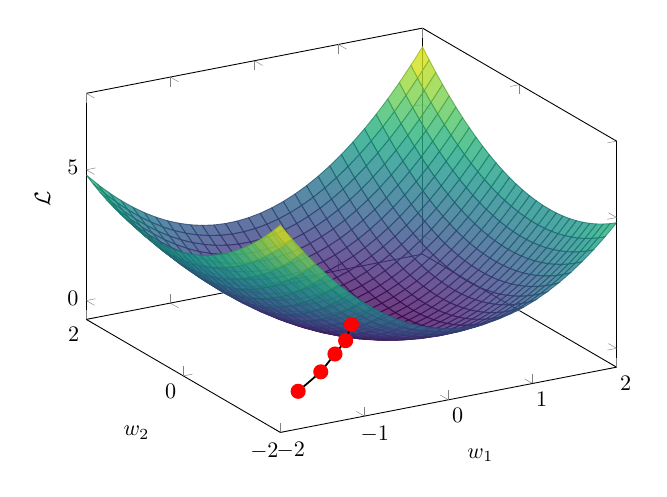
\begin{tikzpicture}[scale=0.8]
        \begin{axis}[
            view={-30}{30},
            xlabel=$w_1$,
            ylabel=$w_2$,
            zlabel=$\mathcal{L}$,
            width=10cm,
            height=8cm
        ]
            % Loss surface approximation
            \addplot3[
                surf,
                colormap/viridis,
                samples=30,
                domain=-2:2,
                opacity=0.8
            ] {x^2 + 0.5*y^2 + 0.3*x*y};
            
            % Gradient descent path
            \addplot3[
                thick,
                black,
                mark=*,
                mark options={red, scale=1.5}
            ] coordinates {
                (-1.5, -1.5, 0)
                (-1.0, -1.1, 0)
                (-0.6, -0.7, 0)
                (-0.3, -0.4, 0)
                (0, 0, 0)
            };
        \end{axis}
    \end{tikzpicture}
    \caption{Gradient descent on a quadratic loss surface}
    \label{fig:gd_quadratic}
\end{figure}

\subsection{Challenges in Optimization}

\begin{itemize}
    \item \textbf{Local Minima:} The loss landscape is non-convex, containing many local minima. However, for large neural networks, local minima are often not a significant problem; saddle points are more common.
    
    \item \textbf{Vanishing/Exploding Gradients:} In deep networks, gradients can become very small (vanish) or very large (explode), making training difficult.
    
    \item \textbf{Plateaus:} Flat regions where gradients are near zero, leading to slow progress.
    
    \item \textbf{Loss Landscapes:} Neural network loss landscapes are complex, with many local minima, saddle points, and flat regions.
\end{itemize}

\begin{figure}[htbp]
    \centering
    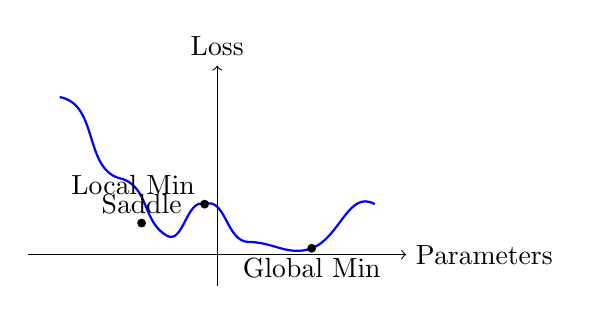
\begin{tikzpicture}[scale=0.8]
        % Drawing a schematic loss landscape
        \draw[->] (-3, 0) -- (3, 0) node[right] {Parameters};
        \draw[->] (0, -0.5) -- (0, 3) node[above] {Loss};
        
        % Loss curve
        \draw[thick, blue] (-2.5, 2.5) to[out=-10, in=170] (-1.5, 1.2) 
            to[out=-20, in=150] (-0.8, 0.3) 
            to[out=-30, in=160] (-0.2, 0.8)  % Local minimum
            to[out=20, in=180] (0.5, 0.2)
            to[out=0, in=200] (1.5, 0.1)  % Global minimum
            to[out=20, in=150] (2.5, 0.8);
            
        % Mark global minimum
        \fill (1.5, 0.1) circle (2pt) node[below] {Global Min};
        
        % Mark local minimum
        \fill (-0.2, 0.8) circle (2pt) node[above left] {Local Min};
        
        % Mark saddle point
        \fill (-1.2, 0.5) circle (2pt) node[above] {Saddle};
    \end{tikzpicture}
    \caption{Schematic of loss landscape with local and global minima}
    \label{fig:loss_landscape}
\end{figure}

\section{Information Theory}

Information theory provides a framework for understanding loss functions, particularly cross-entropy.

\subsection{Entropy}

\begin{definition}[Shannon Entropy]
For a discrete random variable $X$ with probability distribution $p(x)$:
\begin{equation}
H(X) = -\sum_{x} p(x) \log p(x) = E[-\log p(X)]
\end{equation}
Entropy measures the ``uncertainty'' or ``information content'' of a distribution. The logarithm base is typically 2 (bits) or $e$ (nats, natural units).
\end{definition}

\textbf{Historical context:} Claude Shannon introduced entropy in his 1948 paper ``A Mathematical Theory of Communication'' \cite{shannon1948mathematical}, founding information theory. The key insight is that entropy provides the \emph{unique} (up to a constant) measure of uncertainty satisfying natural desiderata: continuity, monotonicity for equiprobable outcomes, and additivity for independent events.

\subsubsection{Proof: \texorpdfstring{$D_{KL}(p \| q) \geq 0$}{D_KL(p || q) >= 0} via Jensen's Inequality}

The non-negativity of KL divergence, one of the most important results in information theory, follows directly from Jensen's inequality.

\begin{theorem}[Jensen's Inequality]
For a convex function $\phi$ and random variable $X$:
\begin{equation}
\phi(E[X]) \leq E[\phi(X)]
\end{equation}
For a concave function, the inequality reverses. Equality holds if and only if $X$ is deterministic (almost surely constant) or $\phi$ is affine on the support of $X$.
\end{theorem}

\begin{proof}[Non-negativity of KL Divergence]
Since $-\log$ is a strictly convex function, by Jensen's inequality:
\begin{align}
-D_{KL}(p \| q) &= \sum_x p(x) \log \frac{q(x)}{p(x)} \\
&= E_{p}\left[\log \frac{q}{p}\right] \\
&\leq \log E_{p}\left[\frac{q}{p}\right] \quad \text{(Jensen's inequality, $\log$ is concave)} \\
&= \log \left(\sum_x p(x) \frac{q(x)}{p(x)}\right) \\
&= \log \left(\sum_x q(x)\right) = \log 1 = 0
\end{align}
Therefore $D_{KL}(p \| q) \geq 0$, with equality if and only if $p = q$ almost everywhere.
\end{proof}

This proof is elegant but powerful: it tells us that the cross-entropy $H(p, q)$ is always at least as large as the true entropy $H(p)$, and the gap is exactly $D_{KL}(p \| q)$.

\begin{figure}[htbp]
    \centering
    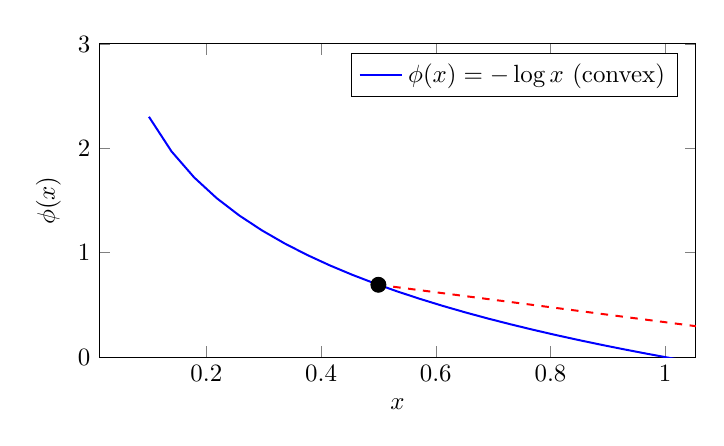
\begin{tikzpicture}[scale=0.9]
        \begin{axis}[
            xlabel={$x$},
            ylabel={$\phi(x)$},
            width=10cm,
            height=6cm,
            domain=0.1:4,
            samples=100,
            legend pos=north east,
            ymin=0, ymax=3,
        ]
            % Convex function (negative log)
            \addplot[thick, blue] {-ln(x)};
            \addlegendentry{$\phi(x) = -\log x$ (convex)}
            % Chord line
            \addplot[thick, red, dashed] coordinates {(0.5, 0.693) (3, -1.099)};
            \node[red] at (axis cs:2.3, 0.4) {Chord (secant line)};
            % Points
            \addplot[only marks, mark=*, mark size=3pt, black] coordinates {(0.5, 0.693) (3, -1.099)};
            % E[X] point on curve
            \addplot[only marks, mark=square*, mark size=3pt, green!60!black] coordinates {(1.75, -0.560)};
            \node[green!60!black] at (axis cs:1.75, -0.9) {$\phi(E[X])$};
            % E[phi(X)] point on chord
            \addplot[only marks, mark=triangle*, mark size=3pt, orange] coordinates {(1.75, -0.203)};
            \node[orange] at (axis cs:1.75, 0.05) {$E[\phi(X)]$};
            % Arrow
            \draw[<->, thick, gray] (axis cs:1.95, -0.560) -- (axis cs:1.95, -0.203);
        \end{axis}
    \end{tikzpicture}
    \caption[Jensen's inequality visualization]{Jensen's inequality for a convex function $\phi(x) = -\log x$: the function evaluated at the mean $E[X]$ lies below the expected value $E[\phi(X)]$.}
    \label{fig:jensen}
\end{figure}

\subsubsection{Mutual Information}

\begin{definition}[Mutual Information]
The mutual information between two random variables $X$ and $Y$ is:
\begin{equation}
I(X; Y) = D_{KL}(p(x, y) \| p(x)p(y)) = \sum_{x,y} p(x, y) \log \frac{p(x, y)}{p(x)p(y)}
\end{equation}
\end{definition}

Mutual information satisfies:
\begin{align}
I(X; Y) &= H(X) - H(X \mid Y) = H(Y) - H(Y \mid X) \\
I(X; Y) &= H(X) + H(Y) - H(X, Y) \\
I(X; Y) &\geq 0 \quad \text{with equality iff } X \perp Y
\end{align}

\textbf{Applications in deep learning:}
\begin{itemize}
    \item \textbf{InfoNCE Loss} (Chapter~3): Contrastive learning maximizes mutual information between augmented views of the same image.
    \item \textbf{Information Bottleneck Theory} \cite{tishby2015deep}: Deep learning is viewed as successive compression of the input $\mathbf{X}$ into representations $\mathbf{T}$ that preserve maximal information about the target $\mathbf{Y}$:
    \begin{equation}
    \min_{p(\mathbf{t}|\mathbf{x})} \; I(\mathbf{X}; \mathbf{T}) - \beta I(\mathbf{T}; \mathbf{Y})
    \end{equation}
    \item \textbf{VAE} \cite{kingma2013auto}: The evidence lower bound (ELBO) can be written as:
    \begin{equation}
    \log p(\mathbf{x}) \geq \mathbb{E}_{q(\mathbf{z}|\mathbf{x})}[\log p(\mathbf{x}|\mathbf{z})] - D_{KL}(q(\mathbf{z}|\mathbf{x}) \| p(\mathbf{z}))
    \end{equation}
\end{itemize}

\begin{property}[Properties of Entropy]
\begin{itemize}
    \item $H(X) \geq 0$ for all distributions
    \item $H(X) = 0$ if and only if $p(x) = 1$ for some $x$ (deterministic)
    \item $H(X)$ is maximized for the uniform distribution
    \item Binary entropy: $H_b(p) = -p\log p - (1-p)\log(1-p)$
\end{itemize}
\end{property}

\subsection{Cross-Entropy and KL Divergence}

\begin{definition}[Cross-Entropy]
For two probability distributions $p$ (true) and $q$ (predicted):
\begin{equation}
H(p, q) = -\sum_{x} p(x) \log q(x) = H(p) + D_{KL}(p \| q)
\end{equation}
\end{definition}

\begin{definition}[KL Divergence]
\begin{equation}
D_{KL}(p \| q) = \sum_{x} p(x) \log \frac{p(x)}{q(x)}
\end{equation}
KL divergence measures the ``distance'' from $q$ to $p$ (not a true metric, as it's asymmetric).
\end{definition}

\begin{property}[KL Divergence Properties]
\begin{itemize}
    \item $D_{KL}(p \| q) \geq 0$ (non-negativity)
    \item $D_{KL}(p \| q) = 0$ if and only if $p = q$
    \item $D_{KL}(p \| q) \neq D_{KL}(q \| p)$ (asymmetric)
\end{itemize}
\end{property}

\begin{example}[Cross-Entropy Loss]
For classification with $N$ samples and $K$ classes:
\begin{equation}
\mathcal{L}_{CE} = -\frac{1}{N}\sum_{i=1}^{N}\sum_{k=1}^{K} y_{ik} \log \hat{y}_{ik}
\end{equation}
where $y_{ik}$ is the ground truth (one-hot) and $\hat{y}_{ik} = \text{softmax}(z_{ik})$ is the prediction.

Minimizing cross-entropy is equivalent to minimizing the KL divergence between the true and predicted distributions, since $H(p)$ is constant for one-hot labels.

\textbf{Derivation of the softmax--cross-entropy gradient:} This is one of the most important derivations in deep learning. For a single sample with true class $c$ (one-hot: $y_c = 1$, $y_{k \neq c} = 0$):
\begin{align}
\mathcal{L} &= -\sum_{k=1}^{K} y_k \log \hat{y}_k = -\log \hat{y}_c = -\log \frac{e^{z_c}}{\sum_j e^{z_j}} = -z_c + \log \sum_j e^{z_j} \\
\frac{\partial \mathcal{L}}{\partial z_k} &= -y_k + \frac{e^{z_k}}{\sum_j e^{z_j}} = \hat{y}_k - y_k
\end{align}
This remarkably clean gradient---prediction minus target---is the cornerstone of classification training. The softmax ``cancels'' with the cross-entropy logarithm, avoiding the numerical issues that plague computing them separately.
\end{example}

\section{Chapter Summary}

This chapter covered the essential mathematical foundations for neural networks:

\begin{enumerate}
    \item \textbf{Linear Algebra:} Vectors, matrices, tensor operations, and norms are the building blocks for representing and manipulating data and parameters in neural networks.
    
    \item \textbf{Calculus:} Derivatives, gradients, and the chain rule are fundamental for computing gradients during backpropagation.
    
    \item \textbf{Probability Theory:} Distributions, expected values, and Bayes' rule provide the framework for understanding predictions and designing loss functions.
    
    \item \textbf{Optimization:} Gradient descent and its variants are the workhorses of neural network training.
    
    \item \textbf{Information Theory:} Entropy and KL divergence justify the use of cross-entropy loss.
\end{enumerate}

These mathematical tools will be applied throughout the textbook as we explore activation functions, loss functions, network architectures, and training algorithms.

\section{Further Reading}

For deeper coverage of these topics:

\begin{itemize}
    \item \cite{bishop2006pattern} - Comprehensive treatment of linear algebra and probability
    \item \cite{strang2009introduction} - Excellent introduction to linear algebra
    \item \cite{cover2012elements} - Classic text on information theory
    \item \cite{kingma2013auto} - Variational inference and the ELBO
    \item \cite{tishby2015deep} - Information bottleneck theory for deep learning
    \item \cite{choromanska2015loss} - Loss surface analysis of neural networks
    \item \cite{goodfellow2016deep} - Chapter 2 covers mathematical foundations for deep learning
    \item \cite{hu2021lora} - Low-rank adaptation and low-rank structure in modern models
\end{itemize}

% ==============================================================================
% EXERCISES
% ==============================================================================

\section{Exercises}

\begin{enumerate}
    \item \textbf{Linear Algebra:} Given a weight matrix $\mathbf{W} \in \mathbb{R}^{256 \times 512}$, how many parameters does this layer have if we include a bias term? Write the computational cost in FLOPs for a single forward pass.
    
    \item \textbf{Calculus:} Compute the gradient $\frac{\partial \mathcal{L}}{\partial \mathbf{W}}$ for a single-layer network with output $\mathbf{y} = \mathbf{W}\mathbf{x}$, where $\mathcal{L} = \|\mathbf{y} - \mathbf{t}\|^2$.
    
    \item \textbf{Probability:} Show that the softmax function is invariant to additive constants: $\text{softmax}(\mathbf{z} + c) = \text{softmax}(\mathbf{z})$ for any constant $c$.
    
    \item \textbf{Optimization:} Implement gradient descent for a simple quadratic function $f(x) = x^2$ and analyze the effect of different learning rates.
    
    \item \textbf{Information Theory:} Prove that $D_{KL}(p \| q) \geq 0$ using Jensen's inequality.
\end{enumerate}
